\chapter{Results and discussion}
\label{ch:results}

This chapter presents the experimental results obtained with the computational pipeline previously defined.
\section{Exploratory PCA of the dataset}
\label{sec:pca_dataset}

In this work, PCA was first used as an exploratory tool to inspect the structure of the Raman dataset before building the classification model. This analysis should be interpreted as descriptive: since PCA is unsupervised, it does not use the tissue labels to determine the components and is therefore not expected to find directions that are optimal for classification. Nevertheless, it is useful before training a predictive model because it shows whether the spectral dataset contains dominant variance patterns and how many components may be needed to obtain a compact representation of the spectra.

For this exploratory stage, PCA was applied to the cleaned dataset after removing non-informative or unreliable labels, namely unlabeled/transparent pixels and artifacts, as described in \Cref{sec:labels-ch4}. Therefore, the PCA included all valid biological tissue classes, independently of the later binary groupings used for ANN classification.

\subsection{Spectral input and centering}
\label{subsec:pca_input_centering}

PCA was applied to the data matrix \(\mathbf{X}\) introduced in \Cref{sec:dimensionality_reduction}. Each row of \(\mathbf{X}\) corresponds to one spectrum and each column corresponds to one of the \(483\) retained Raman-shift variables.

The effect of the centering step, introduced in \Cref{subsec:pca_centering_covariance}, on a single spectrum is shown in \Cref{fig:original_centered_spectrum}.

\begin{figure}[H]
    \centering
    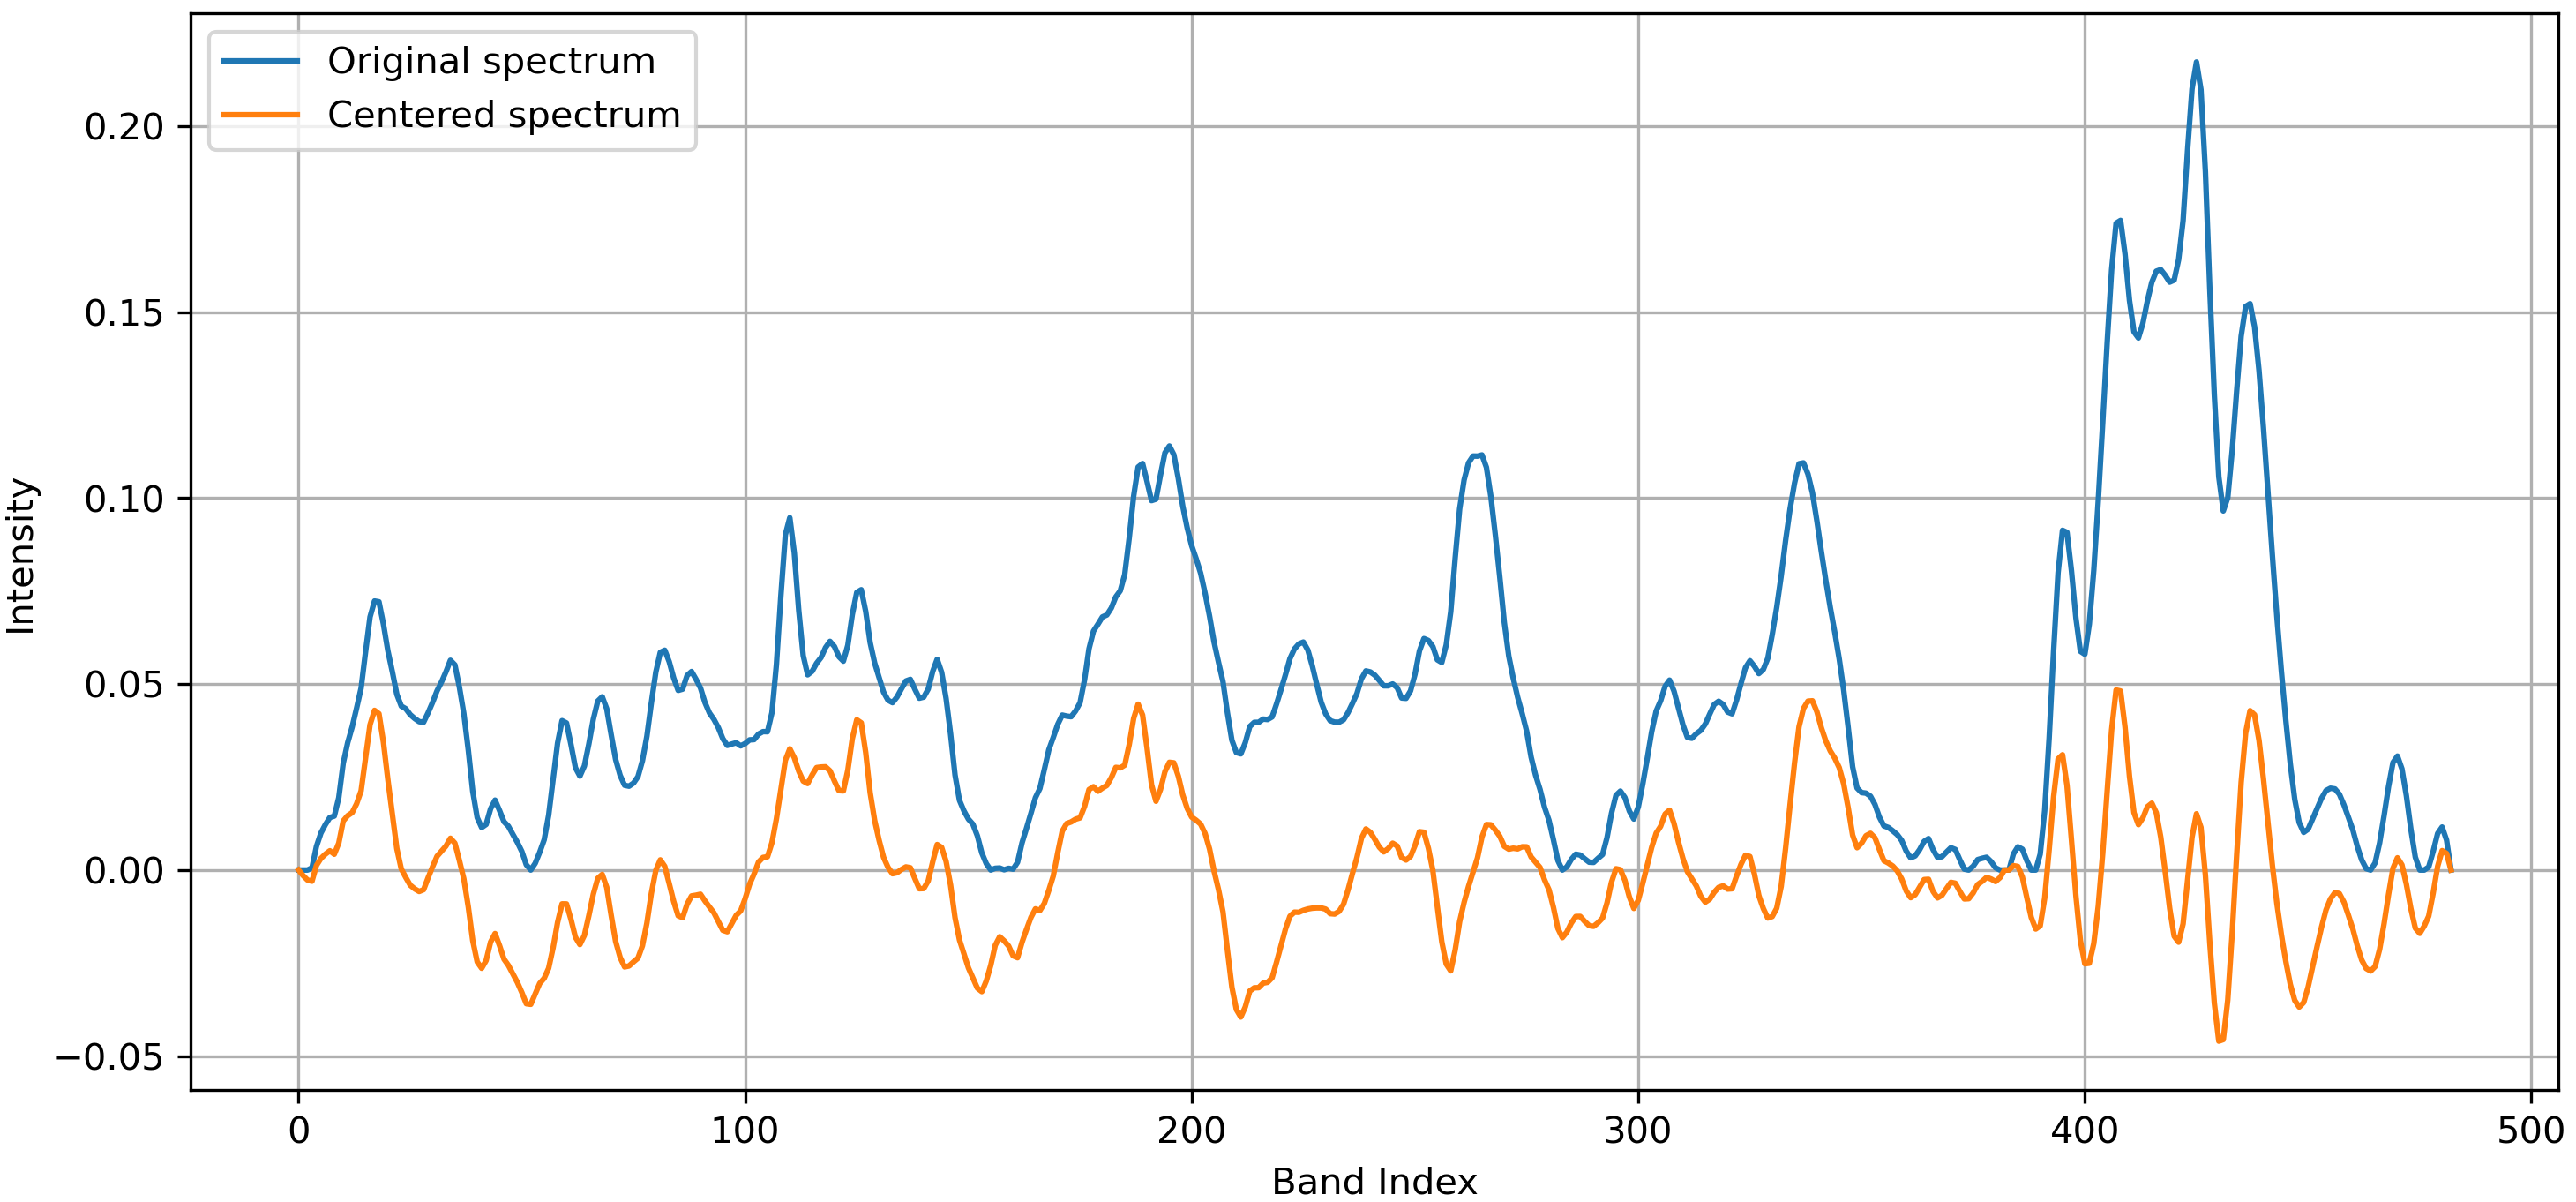
\includegraphics[width=0.65\textwidth]{Images/images_ch_3/05_original_vs_centered_spectrum.png}
    \caption{Example of an original Raman spectrum and the corresponding centered spectrum used for PCA.}
    \label{fig:original_centered_spectrum}
\end{figure}

\subsection{Explained variance of the principal components}
\label{subsec:pca_explained_variance_vibra}

The explained variance was first inspected to evaluate how the information in \(\mathbf{X}\) is distributed across the principal components. The scree plot in \Cref{fig:pca_scree_plot} shows that the first components explain most of the variance, while the contribution of later components rapidly becomes smaller.

\begin{figure}[H]
    \centering
    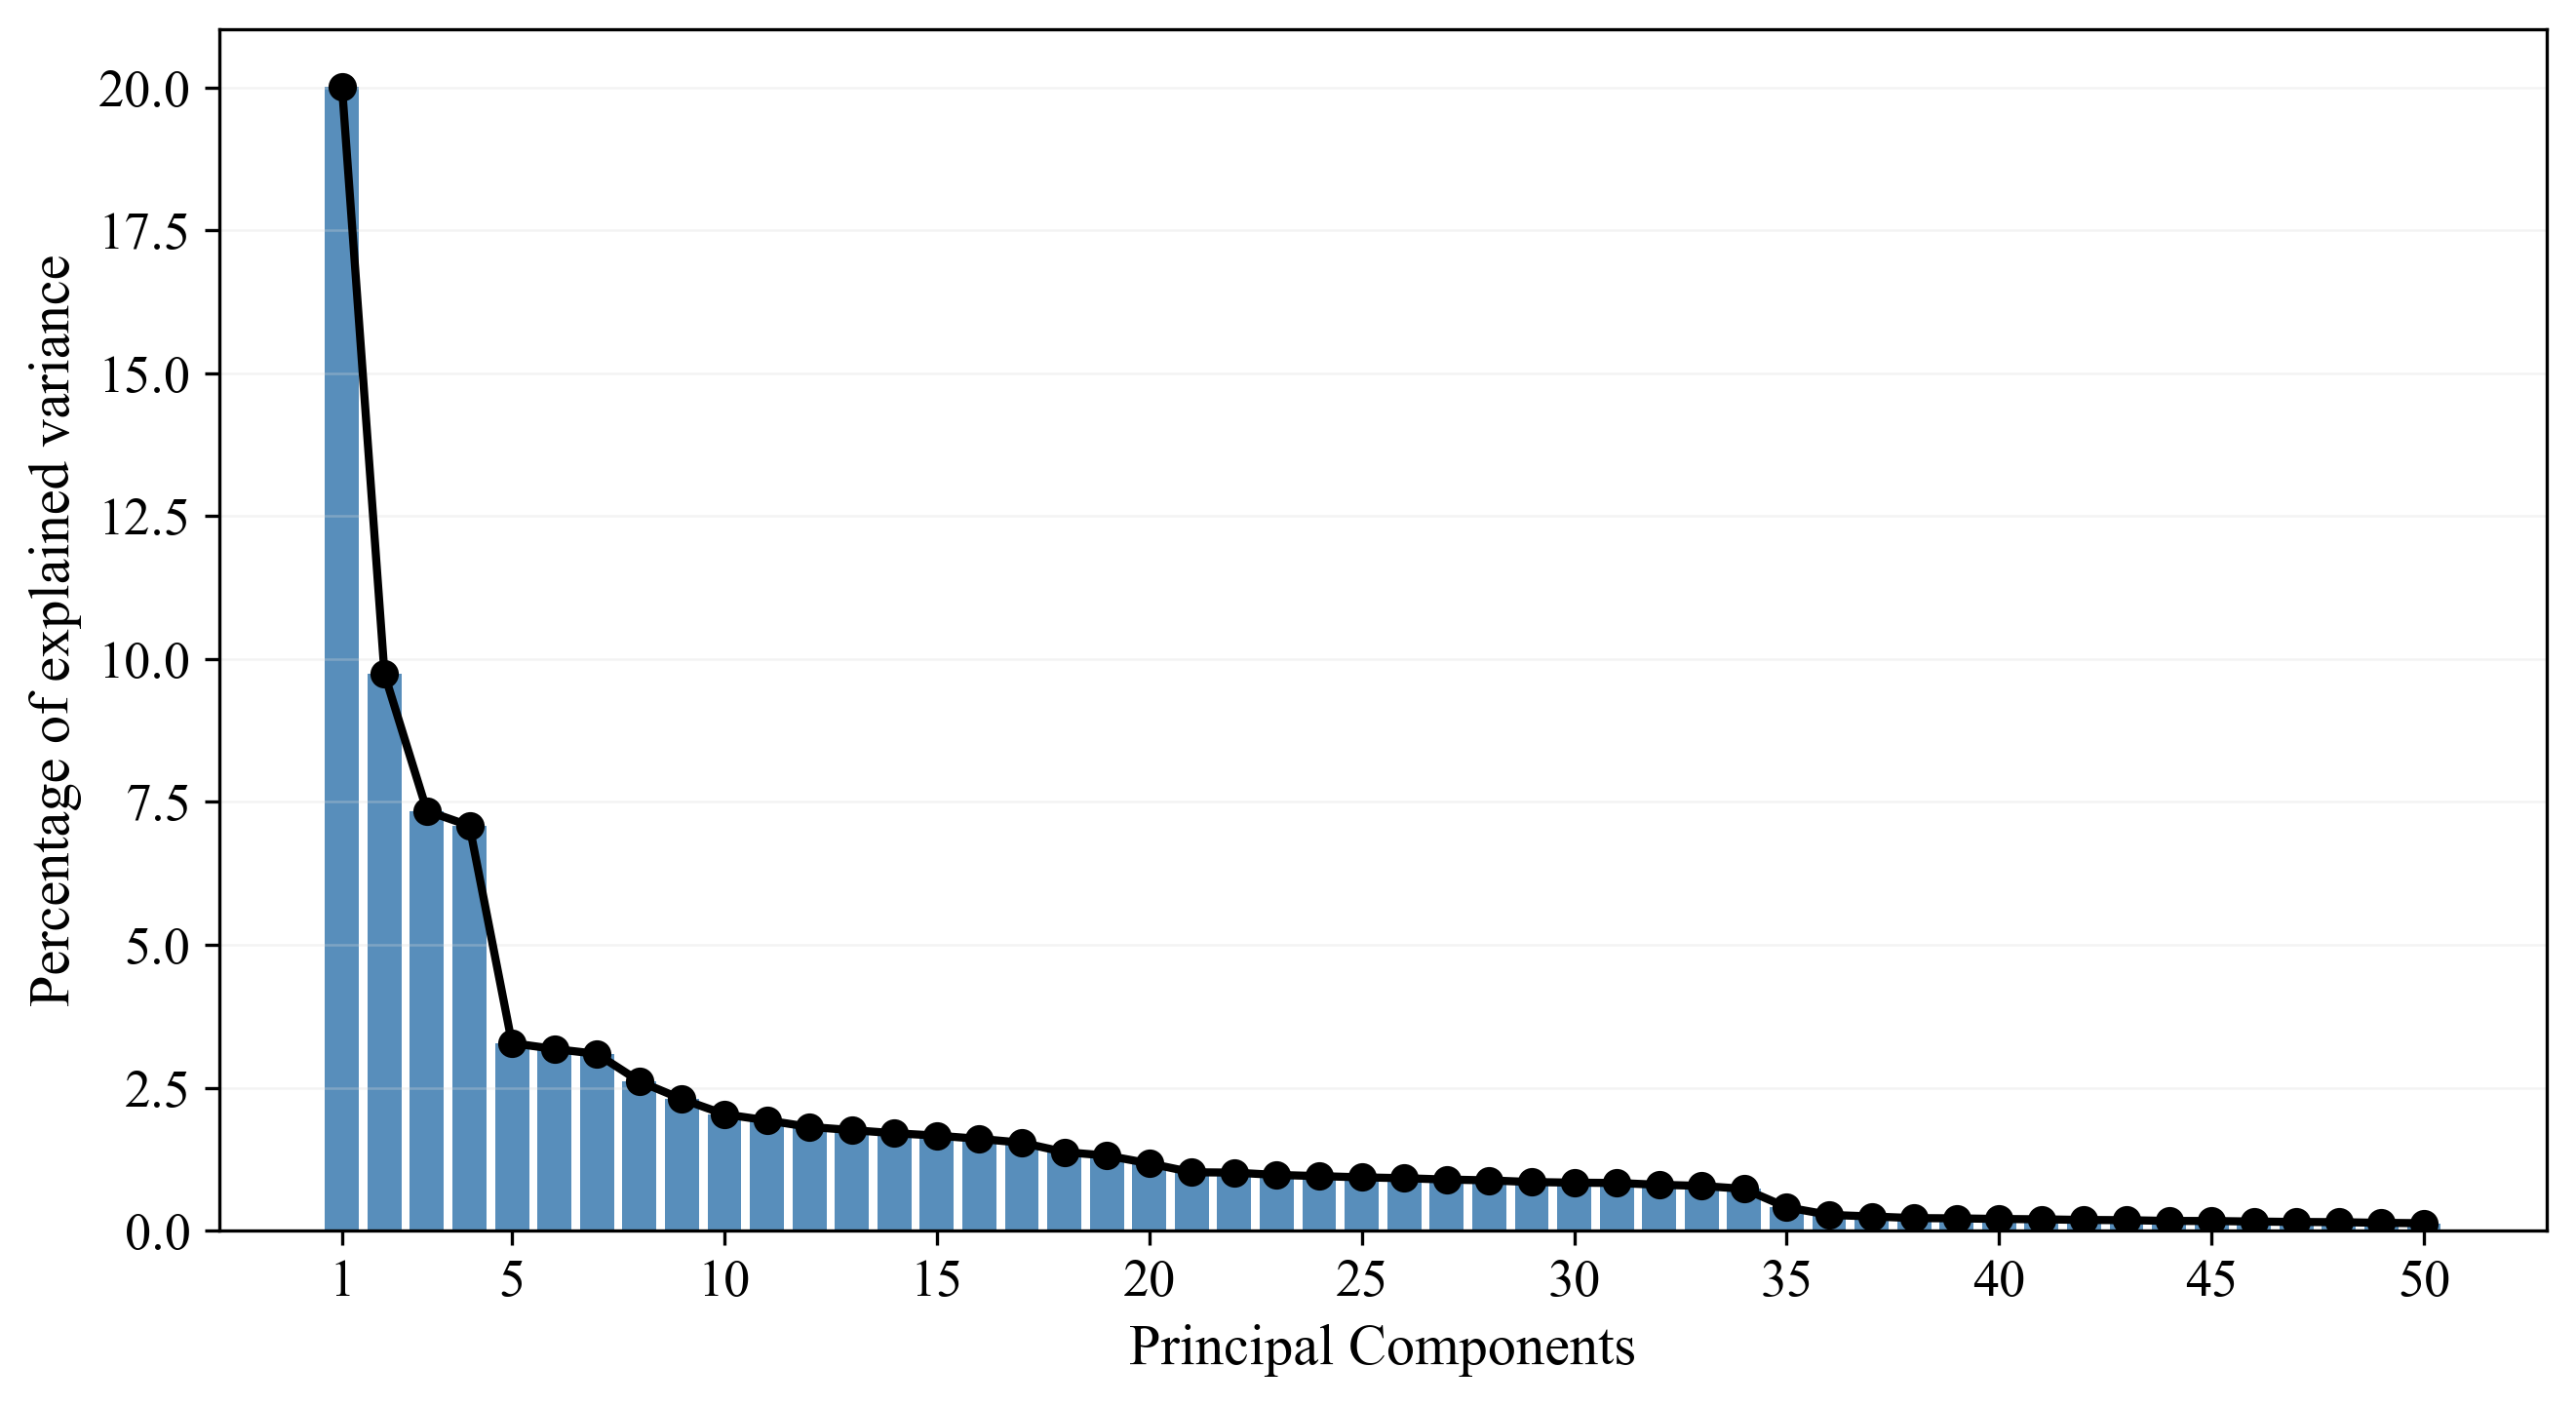
\includegraphics[width=0.65\textwidth]{Images/images_ch_3/07_scree_plot_explained_variance.png}
    \caption{Explained variance associated with the first principal components.}
    \label{fig:pca_scree_plot}
\end{figure}

The cumulative explained variance, shown in \Cref{fig:pca_cumulative_variance}, gives the corresponding global view. The curve has a steep initial increase and then gradually flattens, indicating that the first components retain a large part of the total variance, whereas additional components provide progressively smaller contributions. In this analysis, the \(95\%\) threshold is reached by retaining the first \(89\) principal components; this value was used as a practical reference for comparing reduced PCA representations.

\begin{figure}[H]
    \centering
    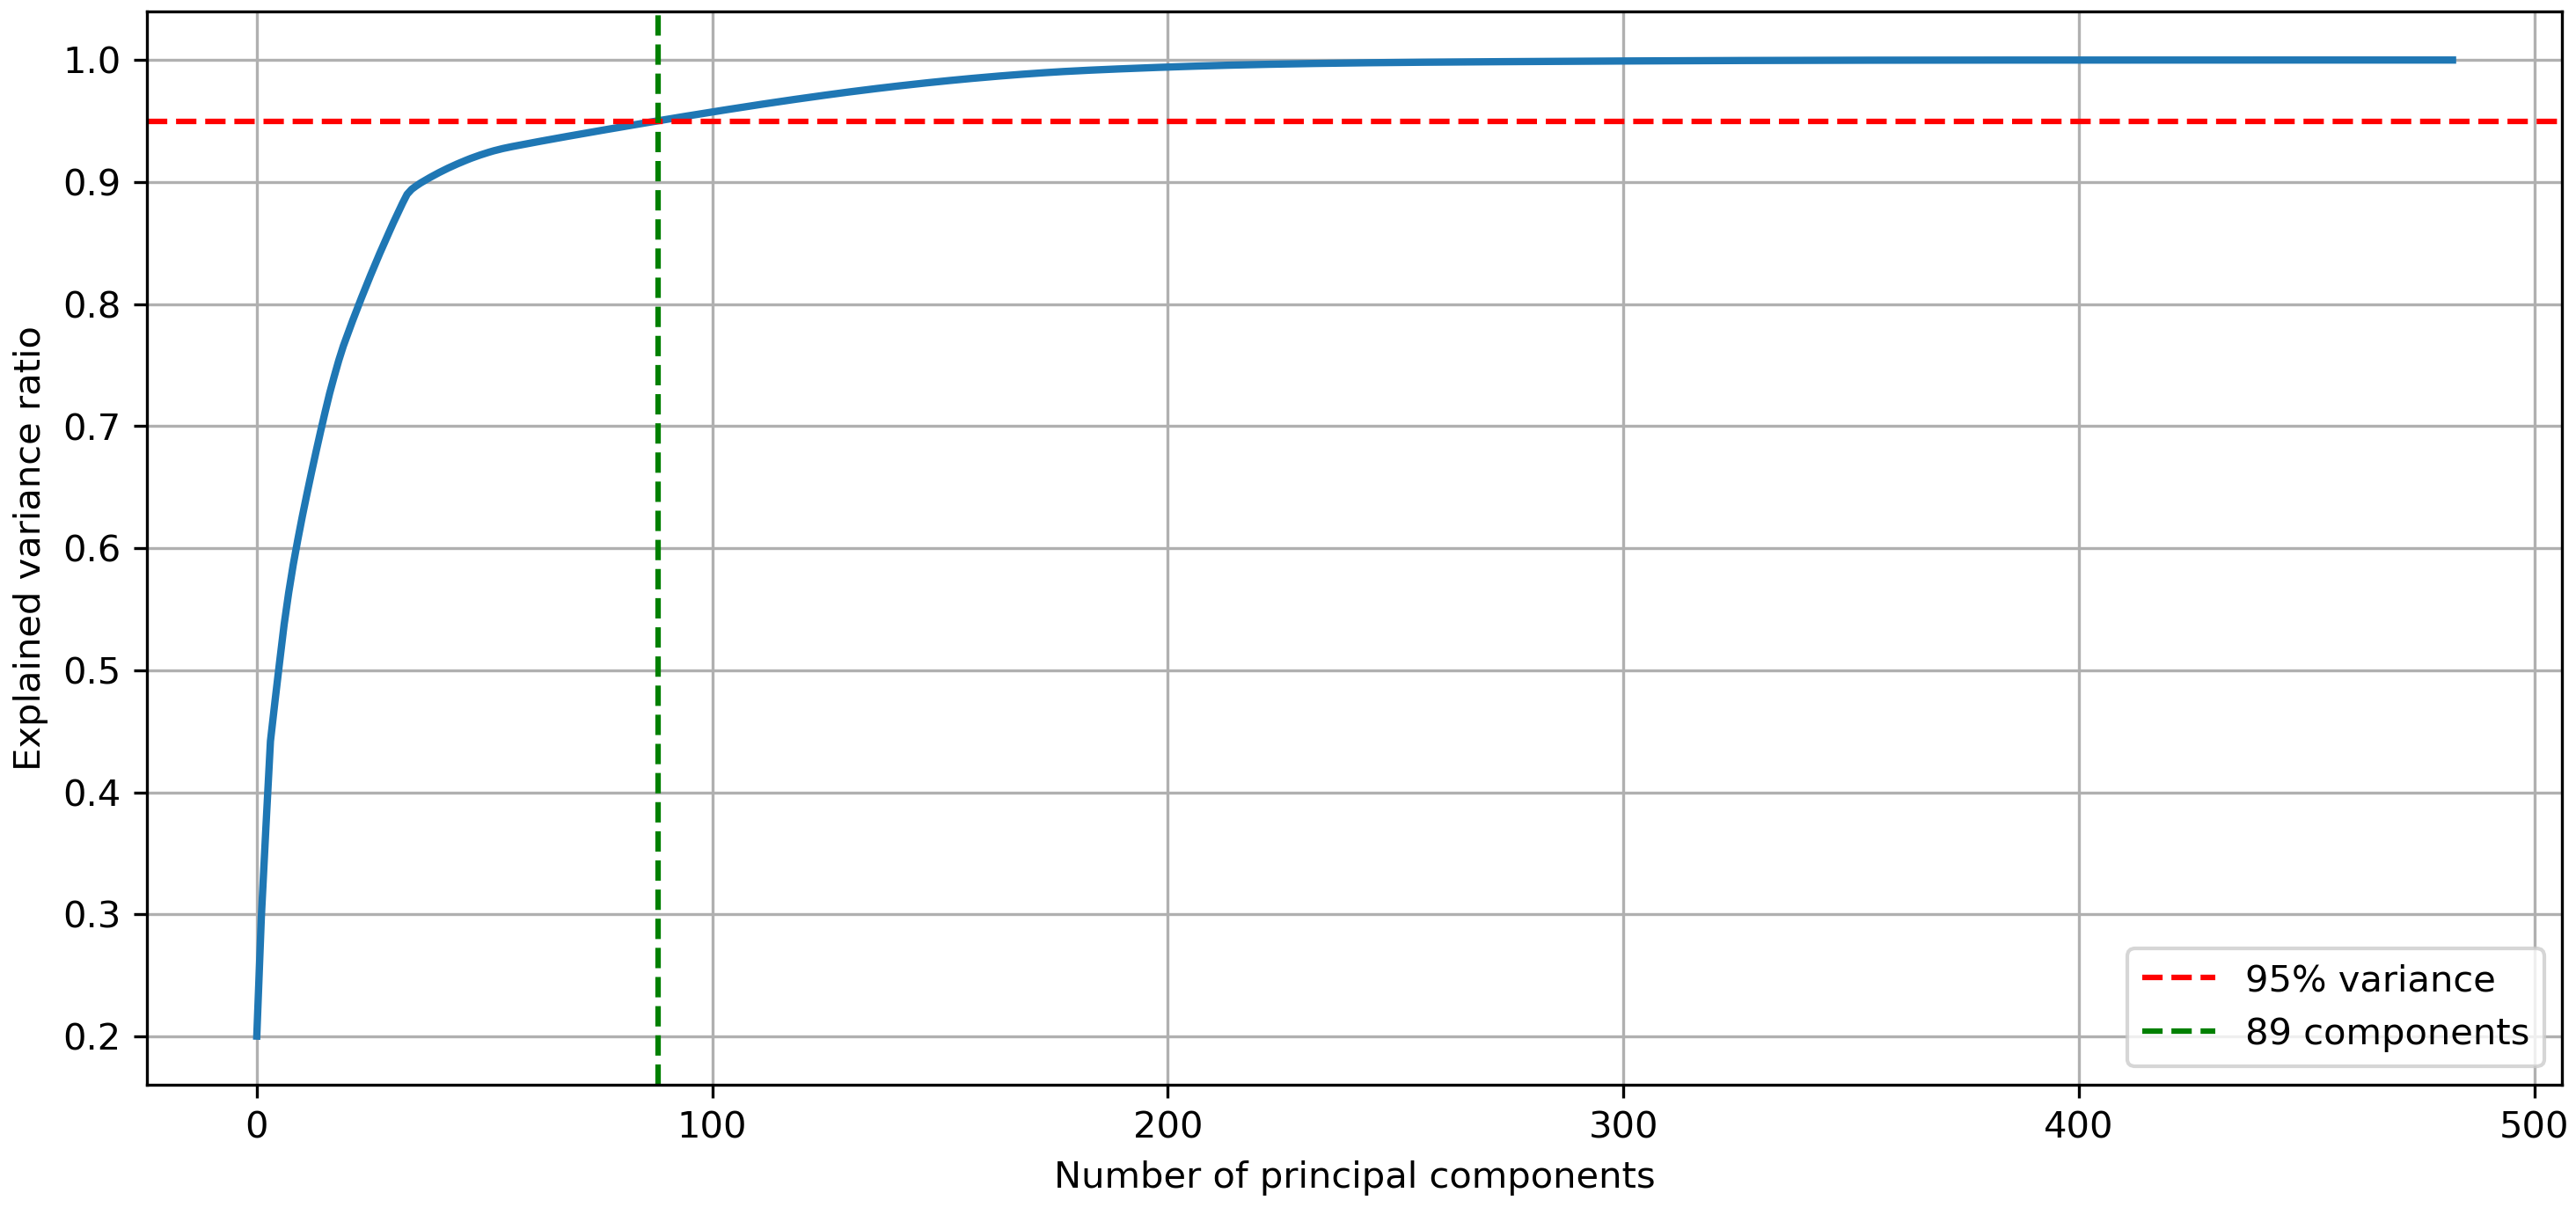
\includegraphics[width=0.65\textwidth]{Images/images_ch_3/06_cumulative_explained_variance.png}
    \caption{Cumulative explained variance as a function of the number of retained principal components.}
    \label{fig:pca_cumulative_variance}
\end{figure}

\Cref{fig:pca_reconstruction_comparison} shows the effect of reconstructing the same spectrum with a very small number of components and with the \(89\) components selected from the cumulative explained variance. The comparison provides a visual interpretation of the dimensionality reduction: a single component captures only the dominant trend, whereas the reconstruction with \(89\) components preserves the main spectral profile.

\begin{figure}[H]
    \centering
    \subfloat[Reconstruction using the first principal component.\label{fig:pca_reconstructed_1}]{
        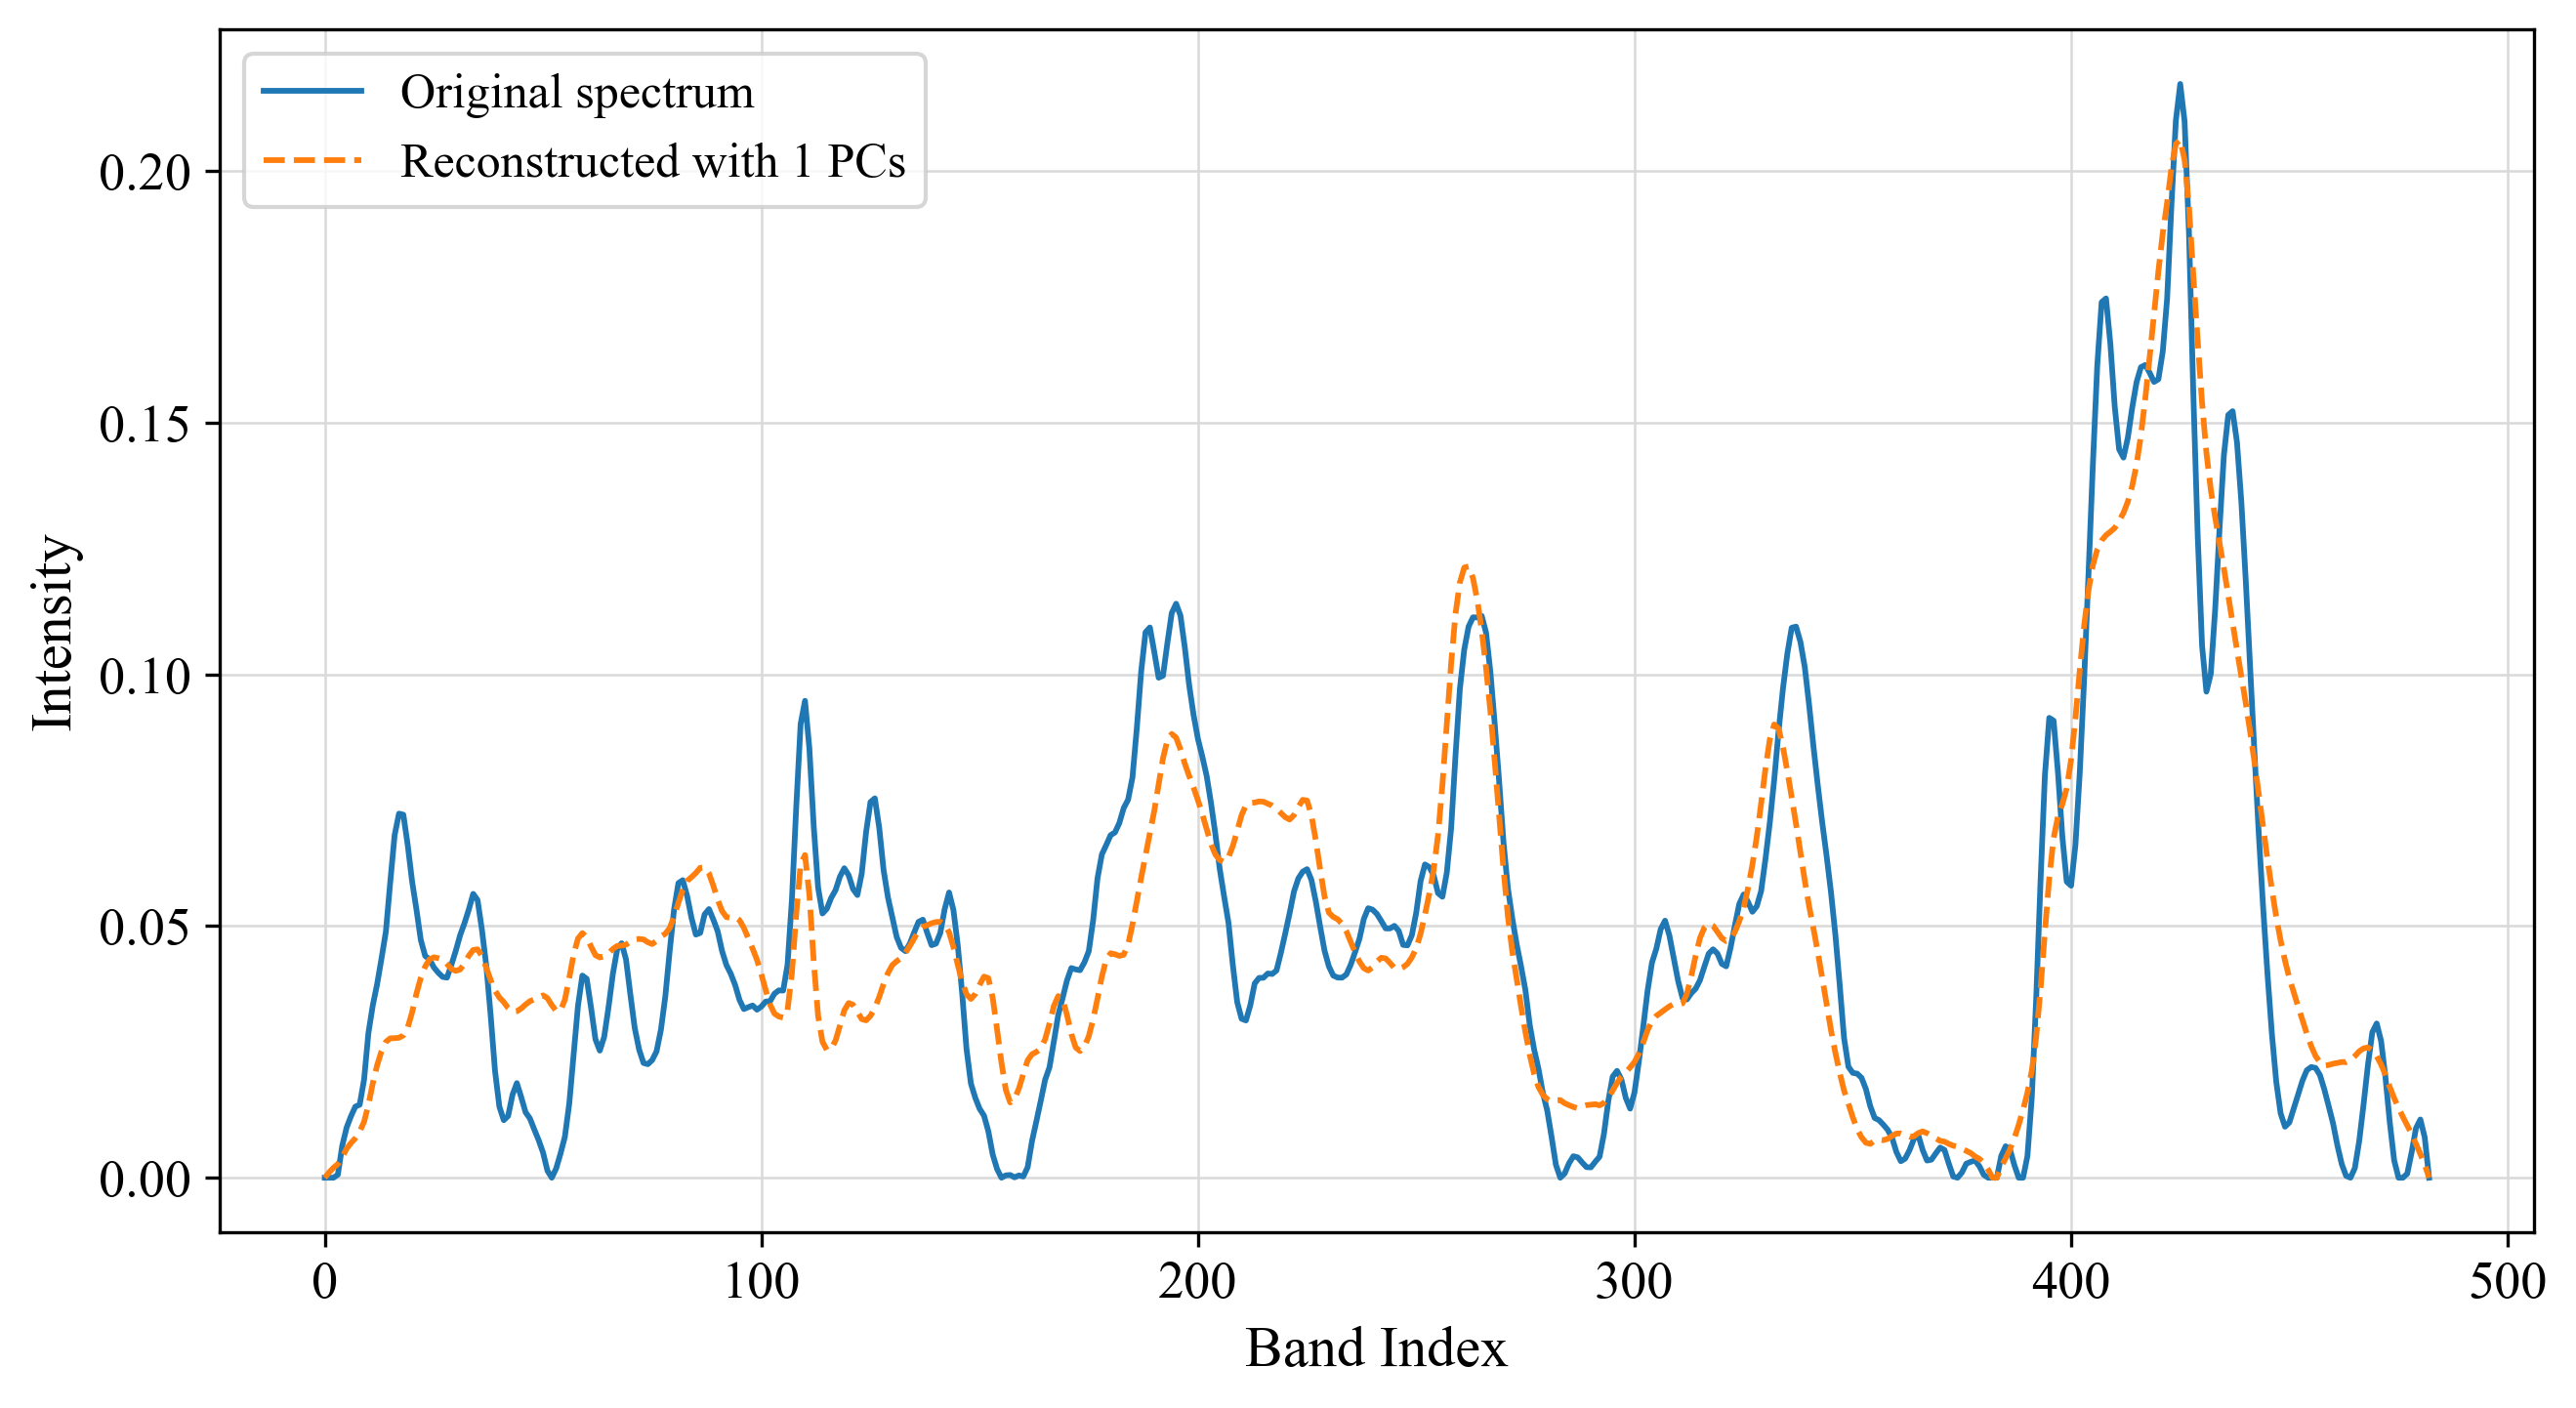
\includegraphics[width=0.48\textwidth]{Images/images_ch_3/12_original_vs_reconstructed_1_components.png}
    }
    \hfill
    \subfloat[Reconstruction using the first \(89\) principal components.\label{fig:pca_reconstructed_89}]{
        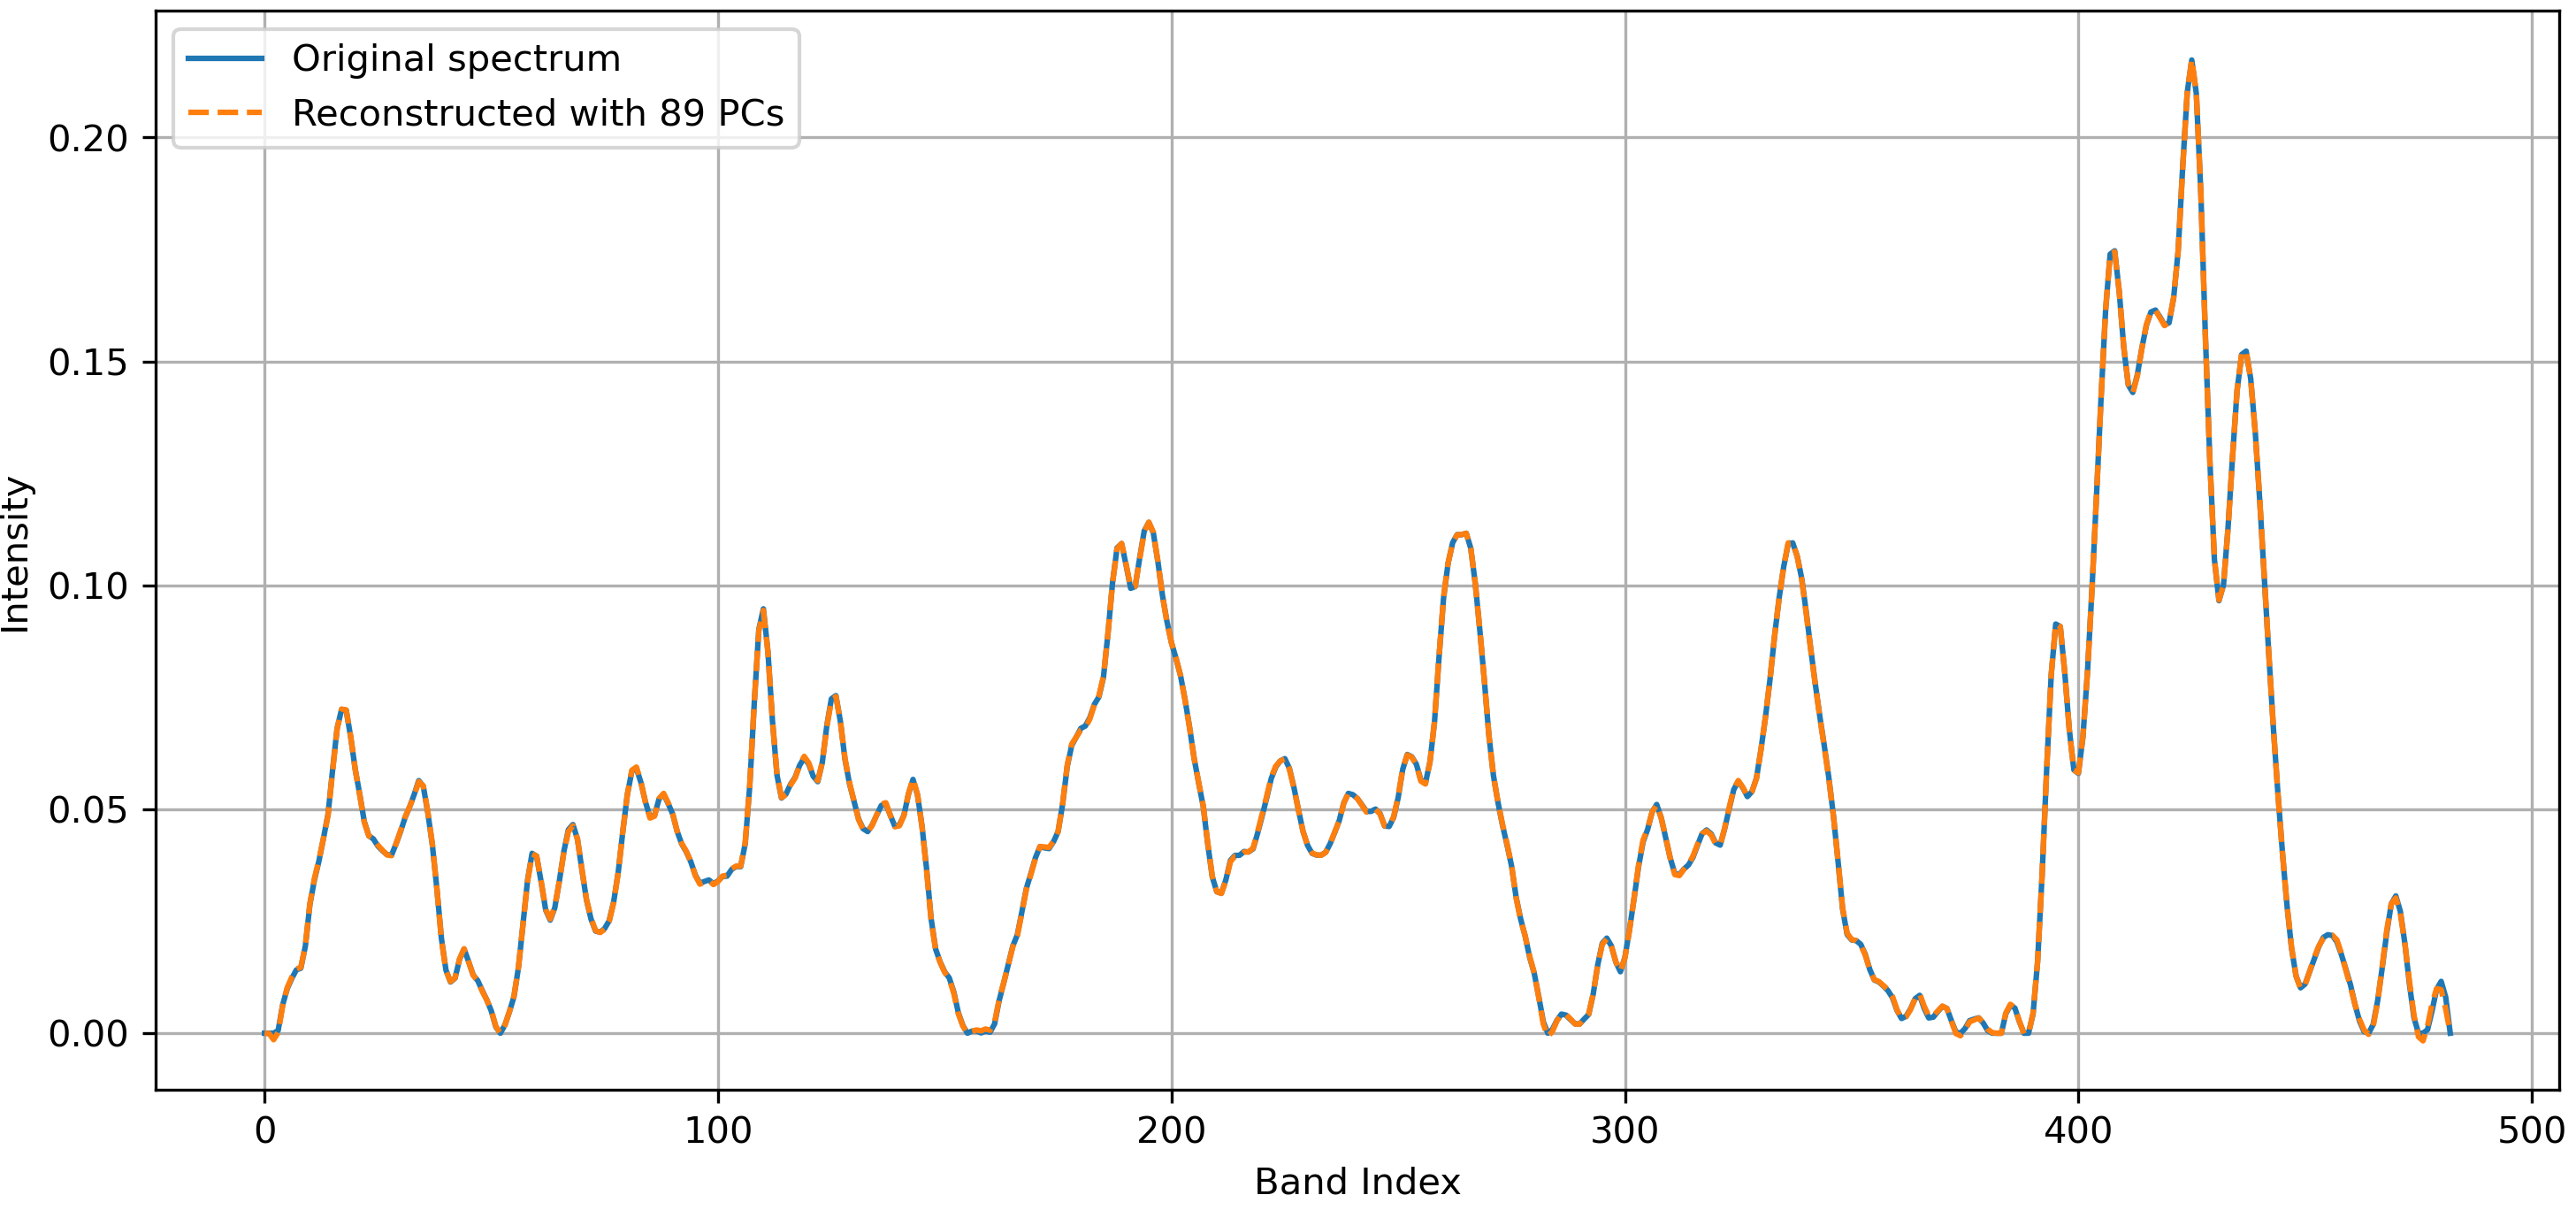
\includegraphics[width=0.48\textwidth]{Images/images_ch_3/12_original_vs_reconstructed_89_components.png}
    }
    \caption{Comparison between an original Raman spectrum and its PCA reconstruction using different numbers of retained principal components.}
    \label{fig:pca_reconstruction_comparison}
\end{figure}

\subsection{Projection of spectra in PCA space}
\label{subsec:pca_projection_vibra}

After inspecting the variance distribution, the spectra were visualized in the PCA space using score plots. For readability, the plots were generated on a random subset of \(10000\) spectra, with points coloured according to the associated tissue label. In these plots, PC1, PC2 and PC483 denote the scores of each spectrum along the corresponding principal components, ordered from the largest to the smallest explained variance.

\begin{figure}[H]
    \centering
    \subfloat[Projection onto PC1 and PC2.\label{fig:pca_score_pc1_pc2}]{
        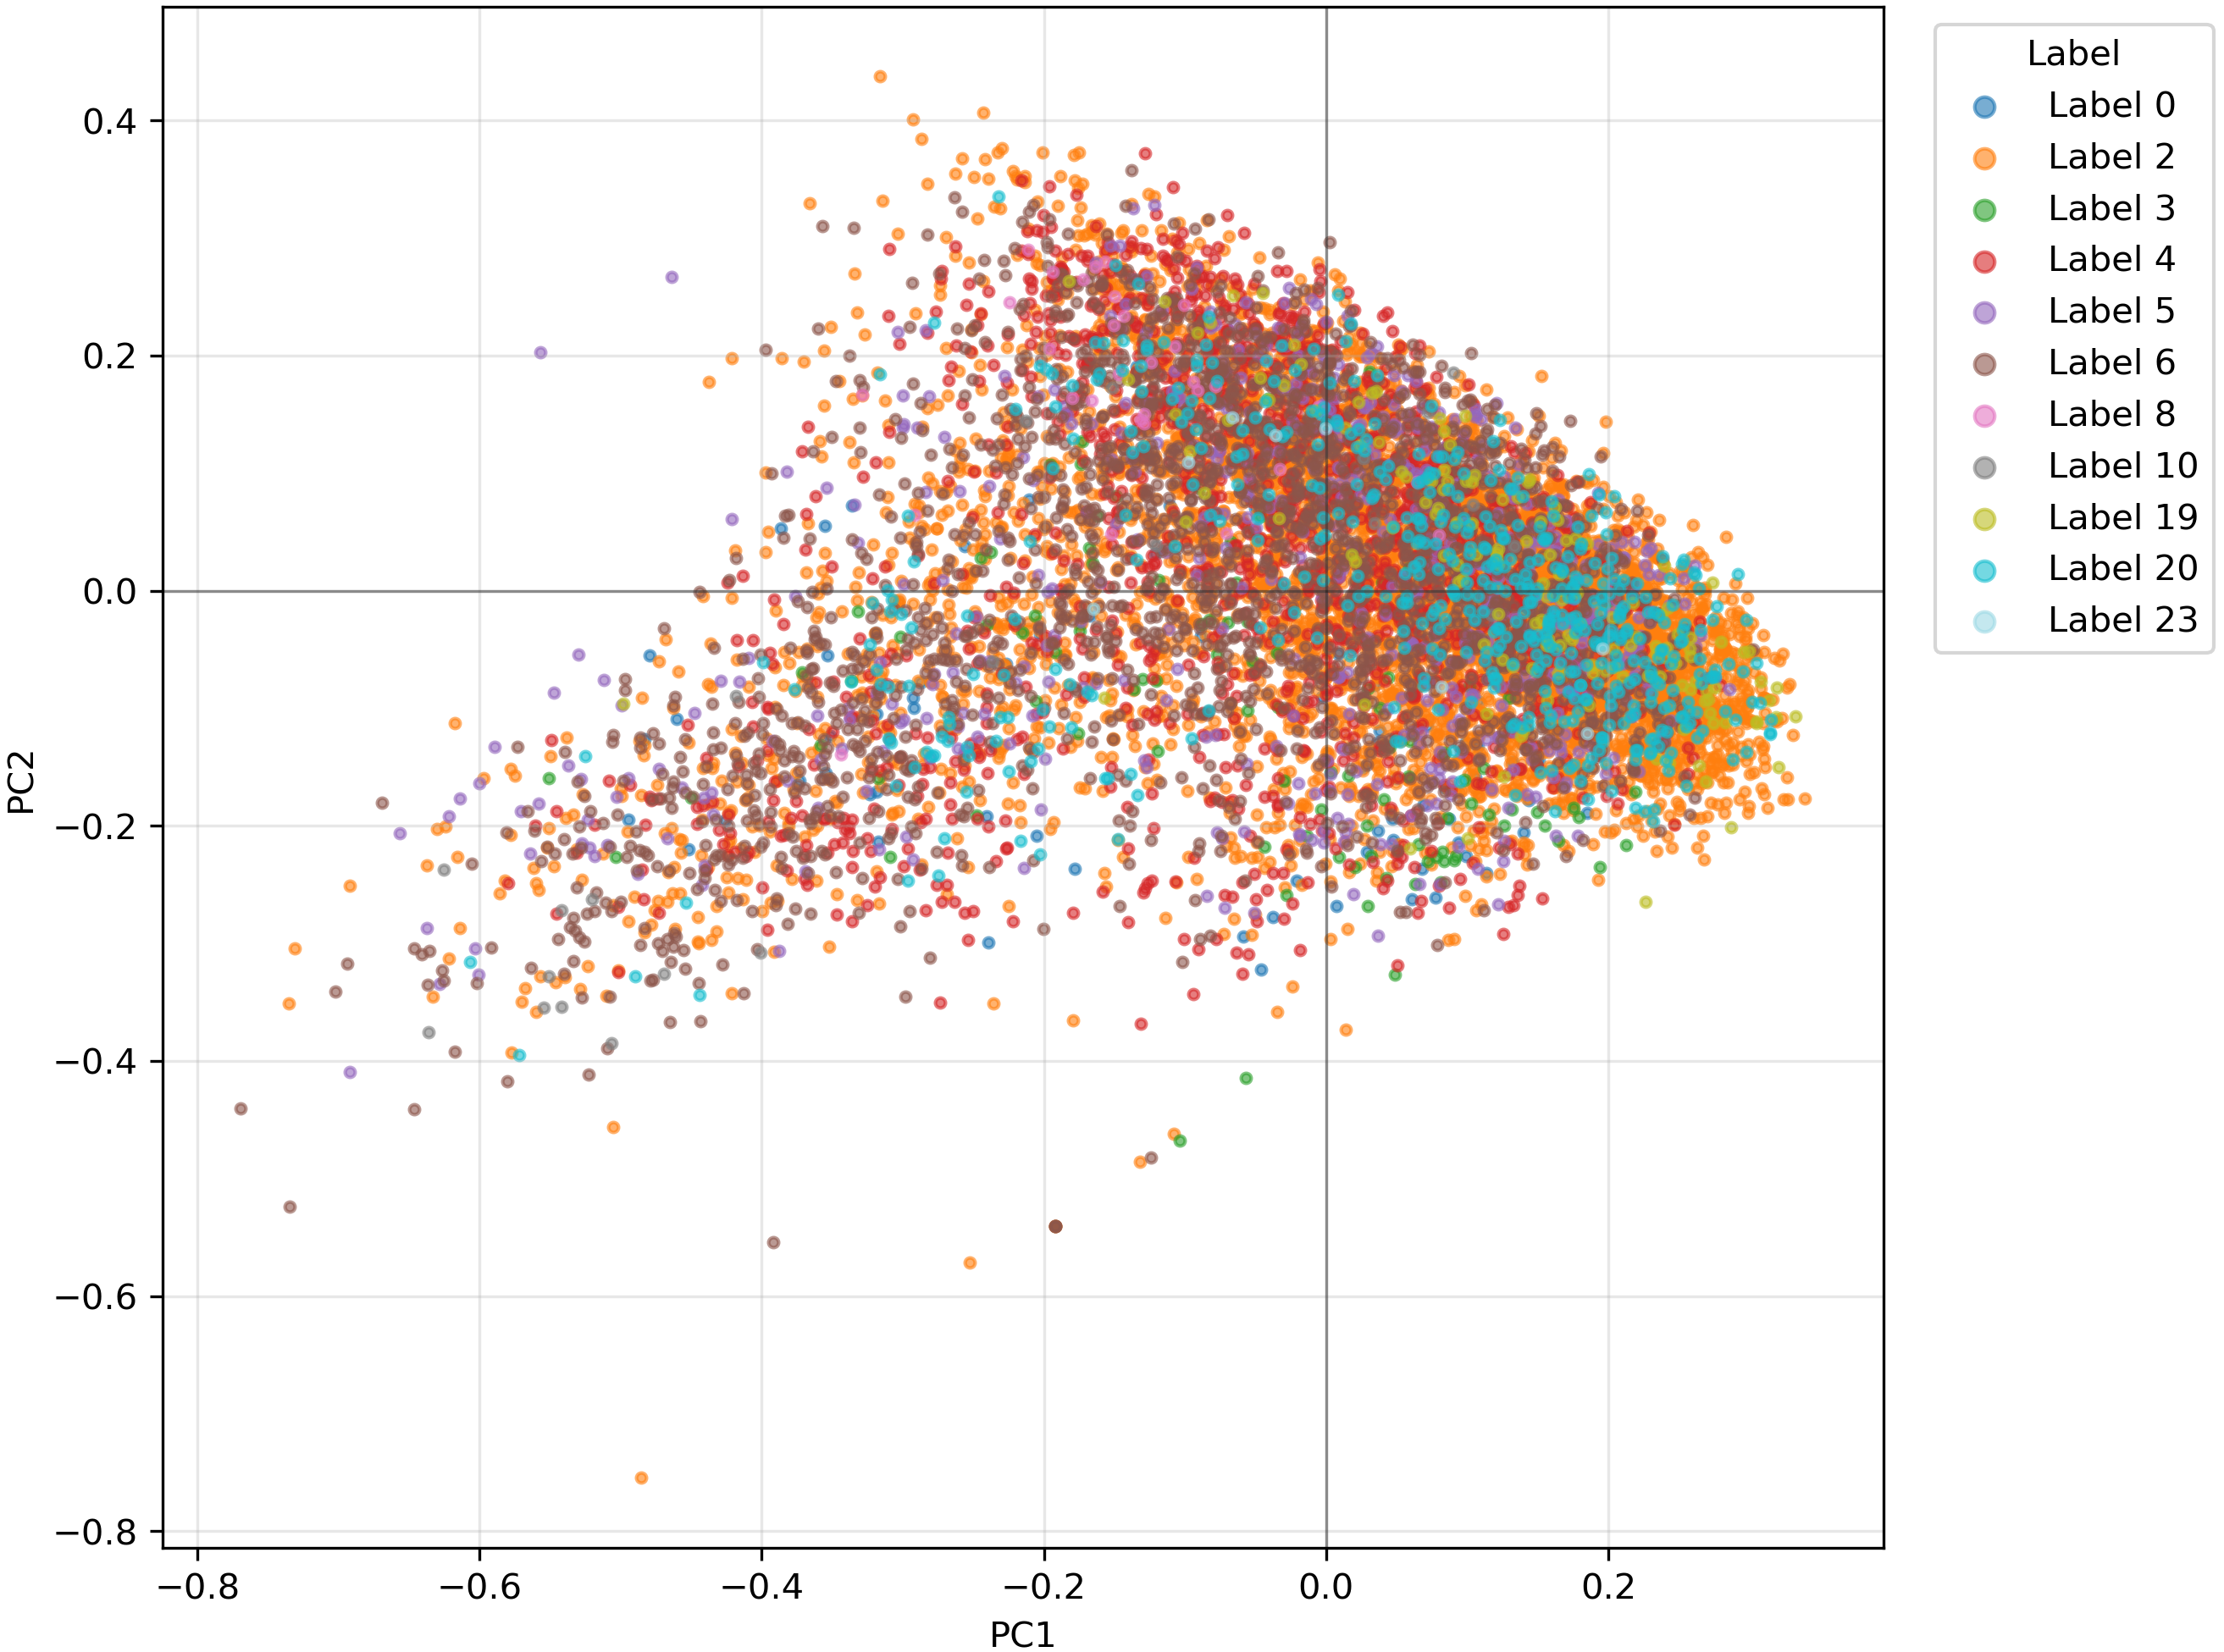
\includegraphics[width=0.48\textwidth]{Images/images_ch_3/08_pca_score_plot_pc1_pc2.png}
    }
    \hfill
    \subfloat[Projection onto PC1 and PC483.\label{fig:pca_score_pc1_pc483}]{
        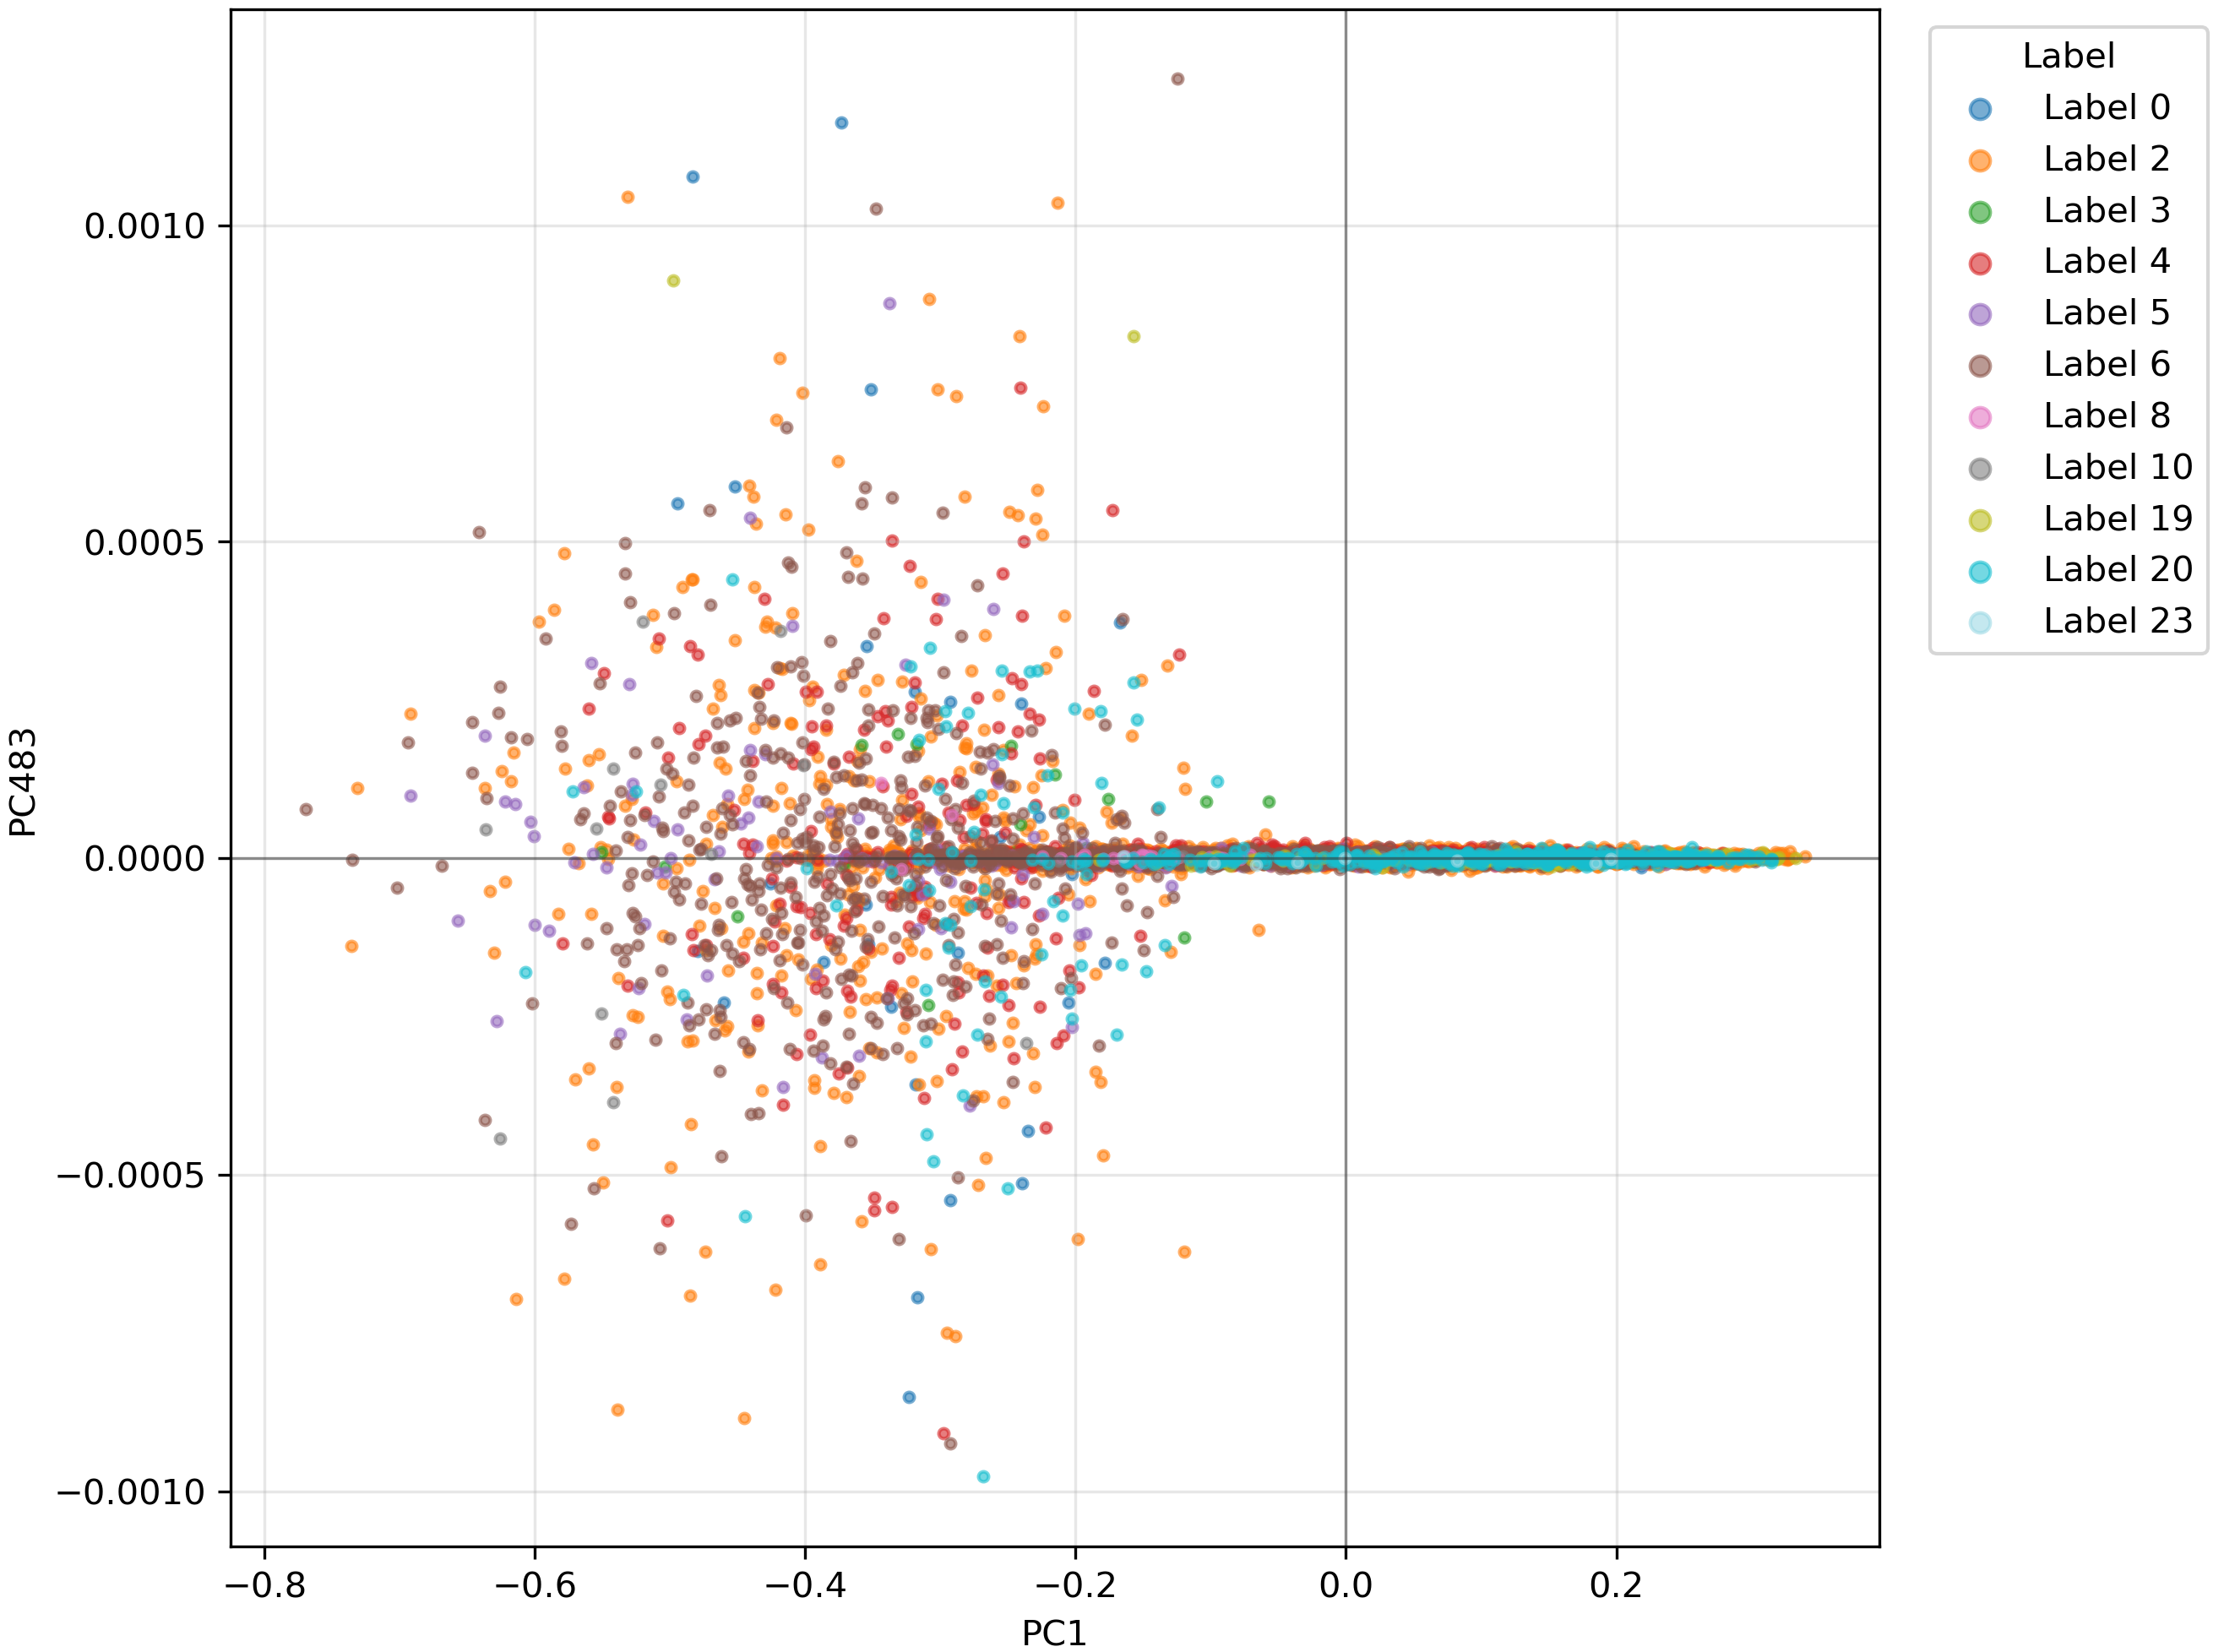
\includegraphics[width=0.48\textwidth]{Images/images_ch_3/09_pca_score_plot_pc1_pc483.png}
    }
    \caption{Score plots of Raman spectra in the PCA space.}
    \label{fig:pca_score_plots}
\end{figure}

\Cref{fig:pca_score_pc1_pc2} shows that the data cloud is distributed along both axes, although its spatial extension is larger along PC1. This is consistent with the larger variance associated with the first principal component, while PC2 still describes a visible part of the variability of the dataset. The coloured labels remain largely overlapped in this plane, indicating that the first two components do not isolate the tissue classes by themselves.

\Cref{fig:pca_score_pc1_pc483} makes the contrast between a dominant component and a late component more evident. The points preserve a wide spread along PC1, whereas their coordinates along PC483 are compressed close to zero. This visual difference reflects the much smaller variance explained by the last component: in this projection, the structure of the point cloud is therefore mainly determined by PC1.

\section{Configuration of the final experiments}
\label{sec:final_experiments_configuration}

The final ANN models were trained for the two binary tasks reported in \Cref{tab:final_binary_experiments}.
\begin{table}[H]
    \centering
    \small
    \renewcommand{\arraystretch}{1.2}
    \begin{tabularx}{\textwidth}{|>{\centering\arraybackslash}p{0.28\textwidth}|>{\centering\arraybackslash}X|>{\centering\arraybackslash}X|}
        \hline
        \textbf{Experiment} & \textbf{Positive class} & \textbf{Negative class} \\
        \hline
        \begin{tabular}[t]{@{}c@{}}Tumour-related class\\vs\\non-tumour\end{tabular} & \begin{tabular}[t]{@{}c@{}}Tumour (2)\\Tumour with necrosis (20)\end{tabular} & \begin{tabular}[t]{@{}c@{}}Valid non-tumour classes\\(0, 3, 4, 5, 6, 8, 10, 19, 23)\end{tabular} \\
        \hline
        \begin{tabular}[t]{@{}c@{}}Tumour-related class\\vs\\stroma\end{tabular} & \begin{tabular}[t]{@{}c@{}}Tumour (2)\\Tumour with necrosis (20)\end{tabular} & Tumour stroma (6) \\
        \hline
    \end{tabularx}
    \renewcommand{\arraystretch}{1}
    \caption{Binary classification experiments evaluated in the final analysis.}
    \label{tab:final_binary_experiments}
\end{table}

In both experiments, the positive class includes tumour and tumour with necrosis, consistently with the definition of the binary classification problems in \Cref{sec:binary_classification-ch4}. The first experiment compares this tumour-related class with tumour stroma, whereas the second compares it with all valid non-tumour tissue classes available in the dataset. The latter setting is broader and more heterogeneous, since its negative class includes multiple histopathological labels.

The final ANN experiments are evaluated in terms of training behaviour, aggregate performance, per-sample variability and the effect of spatial post-processing.

\section{Hyperparameter selection}
\label{sec:hyperparameter_selection}

%check if the title is good or it must be changed

The configuration adopted for the final classification experiments was selected through the hyperparameter search described in \Cref{sec:training-ch4}, which compared different model sizes, numbers of retained PCA components and batch sizes.

The comparison of the tested configurations showed comparable results for all three architectures at equal number of retained PCs. A substantial improvement in the metrics was registered when raising the number of PCs from 1 to 20 for the macro-class problem (\textit{tumor} vs. \textit{healthy}), and a plateau from 20 to 483 PCs. In the single-class problem (\textit{tumor} vs. \textit{tumor stroma}), the metrics improved from 1 to 10, flattening out for bigger dimensionalities, as shown in \cref{fig:heatmap_auc_macroclass,fig:heatmap_auc_singleclass} respectively.

\begin{figure}[H]
    \centering
    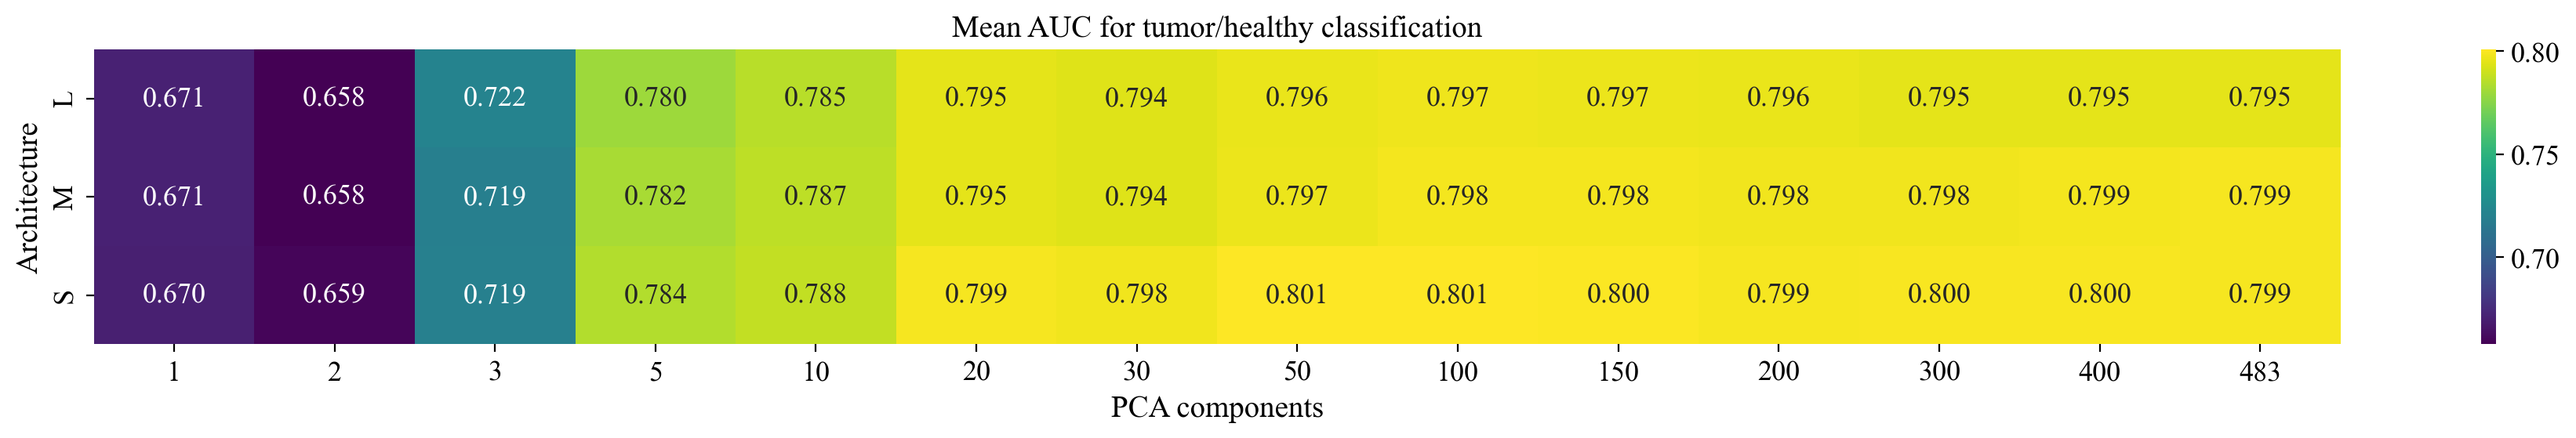
\includegraphics[width=\textwidth]{Images/images_ch_5/heatmap_auc_macroclass.png}
    \caption{AUC across the grid of network architectures and number of retained PCs components for the macro-class problem.  AUC stabilizes for numbers of PCs greater than 20.(\textit{tumor} vs. \textit{healthy}).}
    \label{fig:heatmap_auc_macroclass}
\end{figure}

\begin{figure}[H]
    \centering
    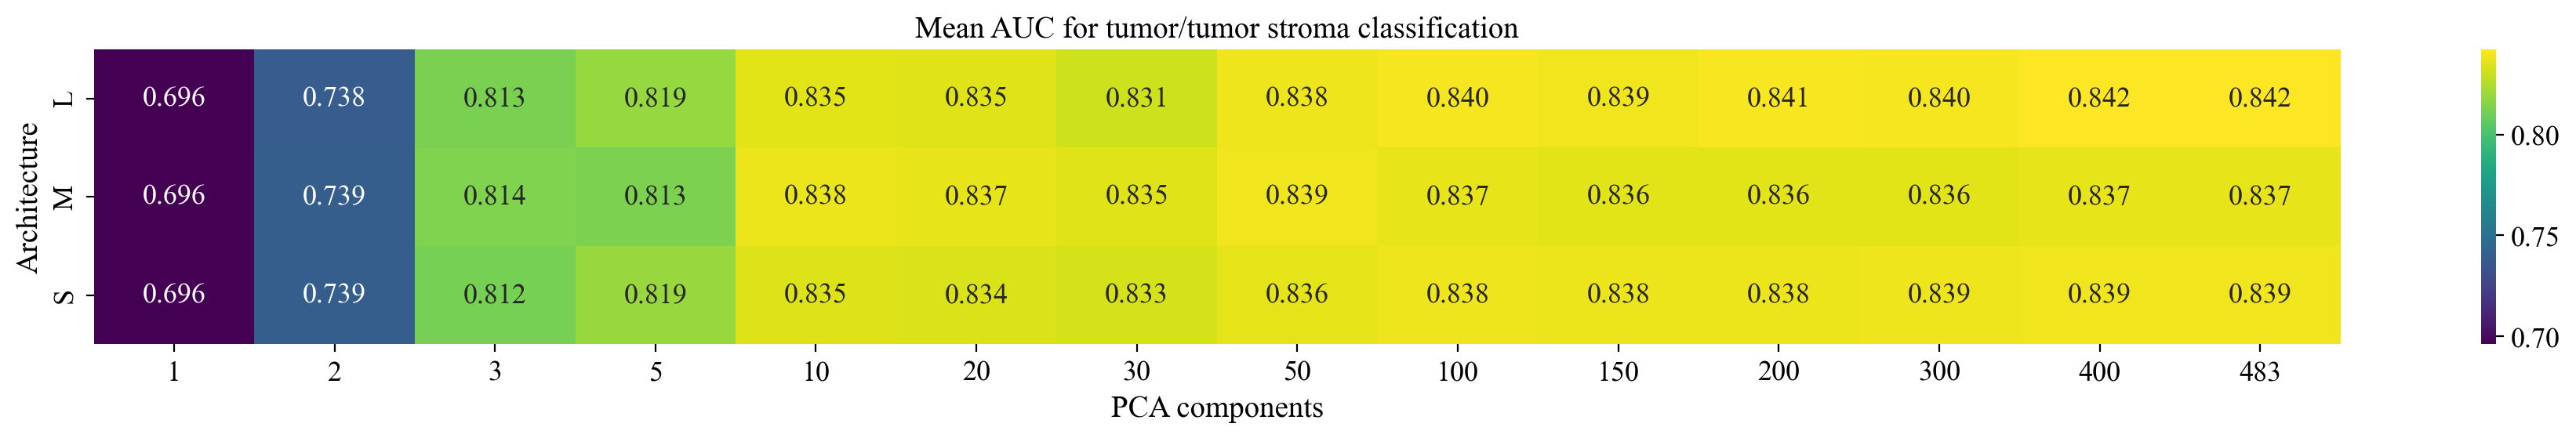
\includegraphics[width=\textwidth]{Images/images_ch_5/heatmap_auc_singleclass.png}
    \caption{AUC across the grid of network architectures and number of retained PCs components for the single-class problem. AUC stabilizes for numbers of PCs greater than 10.(\textit{tumor} vs. \textit{tumor stroma}).}
    \label{fig:heatmap_auc_singleclass}
\end{figure}

Although some configurations with more components or larger networks obtained equally good scores for AUC, their training curves showed less stable behaviour and a larger discrepancy between training and validation performance which also increased with the epochs. These behavior, exemplified by \cref{fig:overfitting_example_L200} is a clear sign of overfitting. The small model, on the contrary, showed similar behaviors in training and validation for all the considered metrics (\cref{sec:aggregated_classification_results}) and was therefore prefered as a final choice.

\begin{figure}[h]
    \centering
    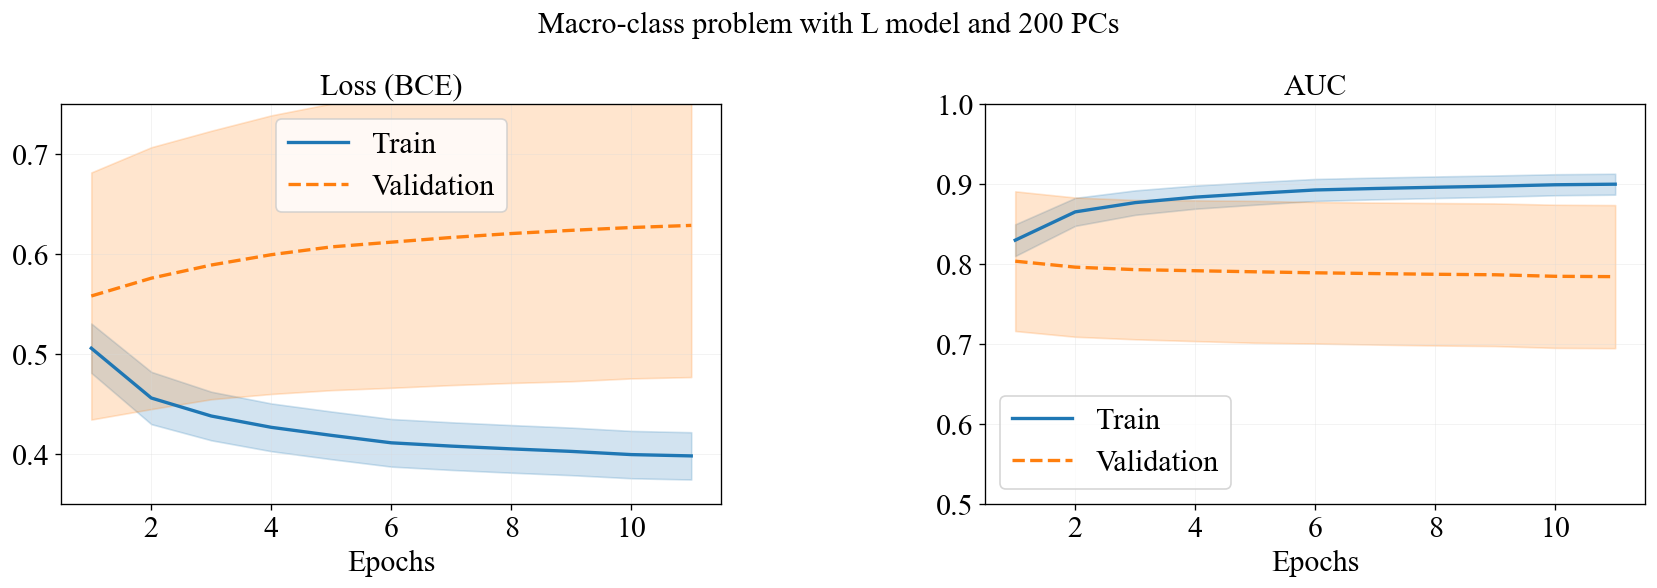
\includegraphics[width=0.7\textwidth]{Images/images_ch_5/overfitting_example_L200.png}
    \caption{Training and validation curves for the large architecture (L) with \(200\) retained PCA components on the macro-class problem (\textit{tumor} vs. \textit{healthy}). The lines show the average value of the metric across 5 folds, while shaded areas display $\pm\sigma$ from the average. The growing separation between training and validation curves is a sign of overfitting.}
    \label{fig:overfitting_example_L200}
\end{figure}

The maximum number of epochs was set to \(100\), although \textit{early stopping} \cref{sec:training-ch4} often halted the training as soon as at epoch 20 due to validation already plateauing. \textit{Early stopping} often acted when prematurely due to noise in the validation curves when working with small batch sizes smaller than 2048. Increasing batch size does in fact average the gradient descent step over more observations, smoothing out the curve and speeding up training, although raising the risk of converging towards sharp minima, which would lead to poor generalization. The final value for the batch size was set as 4096, found to be a good compromise for this task.

The decision threshold used to convert the predicted probability into a binary label was selected empirically by comparing threshold values between \(0.45\) and \(0.50\). The final value was set to \(\tau=0.49\), slightly below the standard threshold of \(0.50\), as it provided a compromise between favouring recall for the positive class and maintaining balanced overall performance. In this application, a false negative, corresponding to a tumour-related spectrum classified as non-tumour, is considered more critical than a false positive, corresponding to a non-tumour spectrum classified as tumour-related. A slightly lower threshold increases the tendency of the classifier to assign spectra to the positive class, supporting recall to tumour-related spectra without excessively penalizing accuracy, as seen in \cref{sec:evaluation_metrics-ch4}.

\begin{table}[H]
    \centering
    \begin{tabular}{|l|c|c|}
        \hline
        \textbf{Hyperparameter} & \textbf{Macro-class} & \textbf{Single-class} \\
        \hline
        Network architecture & \multicolumn{2}{c|}{Small (S)} \\
        \hline
        Retained PCA components & \(20\) & \(10\) \\
        \hline
        Batch size & \multicolumn{2}{c|}{\(4096\)} \\
        \hline
        Decision threshold & \multicolumn{2}{c|}{\(\tau=0.49\)} \\
        \hline
    \end{tabular}
    \caption{Configurations used for the final ANN experiments, for the macro-class (\textit{tumor} vs. \textit{healthy}) and single-class (\textit{tumor} vs. \textit{tumor stroma}) problems.}
    \label{tab:selected_hyperparameters}
\end{table}


\section{Aggregated classification results}
\label{sec:aggregated_classification_results}

The configurations chosen for the two approaches, listed in \cref{tab:selected_hyperparameters} were further analized to asses their effectiveness.

The confusion matrixes and ROC curves showed good results for both problems. The macro-class approach performed slightly below the single-class one, especially in non-tumoral classification (True negatives scores equaled 0.71 and 0.75 respectively). This is a direct consequence of the internal heterogeneity for the healthy class.

%talk about roc and auc per sample

%show graphs of CM, roc, auc


The training behavior was observed to be 
The curves for the single class improved regularly in the early stages of training until reaching a plateau after $\sim20$ epochs on average.

%talk more about curves and show curves

\textbf{Writing notes.} This section should report the quantitative performance obtained across folds. Here the two experiments should probably be compared in parallel, using the same metrics.

\begin{itemize}
    \item Insert a table with fold-wise results and mean \(\pm\) standard deviation for each experiment.
    \item Report the main evaluation metrics introduced in \Cref{sec:evaluation_metrics-ch4}.
    \item Insert the aggregated confusion matrix for each experiment.
    \item Discuss the variability across folds, not only the average values.
    \item Highlight whether the broader tumour vs non-tumour task is harder than the more specific tumour vs stroma task.
\end{itemize}


\section{Per-sample analysis}
\label{sec:per_sample_analysis}

\textbf{Writing notes.} This section should move from global pixel-wise performance to the behaviour observed on individual samples.

\begin{itemize}
    \item Report per-sample metrics or rankings, if available.
    \item Identify representative easy and difficult samples.
    \item Comment on whether errors are concentrated in specific samples or distributed across the dataset.
    \item When prediction maps are shown, use them to connect numerical performance with spatial behaviour inside the Raman maps.
    \item Keep the comparison between the two experiments focused on differences that are visible at sample level.
\end{itemize}

\section{Effect of spatial smoothing}
\label{sec:effect_spatial_smoothing}

\textbf{Writing notes.} This section should evaluate the post-processing step described in \Cref{sec:spatial_post_processing-ch4}.

\begin{itemize}
    \item Compare raw and smoothed predictions for both experiments.
    \item Report whether smoothing improves the selected metrics and whether the effect is consistent across folds or samples.
    \item Insert representative prediction maps before and after smoothing.
    \item Discuss the qualitative effect on maps: reduction of isolated noisy pixels, improved spatial coherence, possible loss of small regions or propagation of local errors.
    \item Keep clear that smoothing is applied after inference and is not part of the ANN training.
\end{itemize}

\section{Interpretation and comparison with the literature}
\label{sec:interpretation_literature}

\textbf{Writing notes.} This section should interpret the results without turning into a new literature review.

\begin{itemize}
    \item Summarize what the results suggest about Raman spectra as inputs for tumour recognition.
    \item Compare the two experiments in terms of biological and computational difficulty.
    \item Relate the observed performance to the spectral complexity and class heterogeneity discussed in the previous chapters.
    \item Add a short comparison with similar Raman spectroscopy and machine learning studies, if useful.
    \item Avoid overclaiming clinical validity: the results support the feasibility of the pipeline on the available dataset.
\end{itemize}

\section{Limitations of the study}
\label{sec:limitations_study}

Although being based on a large dataset (>1000000 observations), the spectra are strongly spatially correlated. This leads to a substantial reduction in useful independent information. The samples are in fact very few (25), with many types of biological tissue being largely underrepresented. The performance, as seen in \cref{sec:per_sample_analysis}, varies depending on the selected samples. A different dataset split or a larger pool of patients and samples may lead to different results compared to what was found in this thesis, which would be a sign of poor generalization.

Another limitation stems from acquisition and preprocessing. The ANN received spectra which underwent a specific pipeline before being suitable for computational analysis. Different choices for the treatment of the samples, instrumentation, acquisition parameters, or preprocessing steps would reflect on the spectral trends. These differences may transfer to the ANN classification problem, altering the final results. The extent of these changes was not assessed in this thesis, which limits how confidently the pipeline can be expected to generalize to spectra acquired under different conditions.

Spatial smoothing was applied as a post-processing step to improve performance due to common isolated label mismatches. Due to not being an internal part of the ANN decision process, it may also suppress real isolated healthy/tumoral regions as it does with noise. Implementing spatial convolution directly into the ANN could thus lead to more precise classification.

\section{Future developments}
\label{sec:future_developments}

Possible developments of this work could revolve around solving the issues listed in \cref{sec:limitations_study}. This would mean broadening the training pool in terms of both samples and patients, as well as quantifying the influence of different experimental conditions and preprocessing on the final result.

Enlarging the training pool would also increase the number of samples available for the underrepresented biological tissue classes, allowing different binary classifications to be explored. Multiclass classification would be particularly useful, allowing faster, in-vivo and pixel-exact tissue identification, now performed through H\&E staining by a histopathologist.

Further improvements in the deep learning pipeline may be implemented through a convolutional neural network (CNN). Spectral convolution (1D) could lead to better identification of specific peaks and patterns associated with biological signatures. Spatial convolution (2D) on the Raman maps could serve a similar purpose to spatial smoothing, but inside the deep learning pipeline instead of as a heuristic post-processing step.